The intermediate latency between a client and a data centre is a product of propagation, modulation, and network routing and traffic shaping. Propagation is a clear physical obstacle to reducing latency, and there is very little evidence to suggest that information will propagate faster than $\frac{2}{3}$ of the speed of light, at scale, in the near future. Furthermore, the delay in the backbone network is incurred to the most part by routing. A full point to point network where the propagation speed is the only limit, is not economically viable and would dissolve the fabric of the Internet. As such, we can always expect a certain amount of network contributed latency and jitter. At best, an LTE mobile access network adds about 5 ms of latency \cite{blajic2006latency}. Radio access network latency can be expected to diminish over the next few generations of mobile networks. 

\begin{figure}[tb]
	\centering
	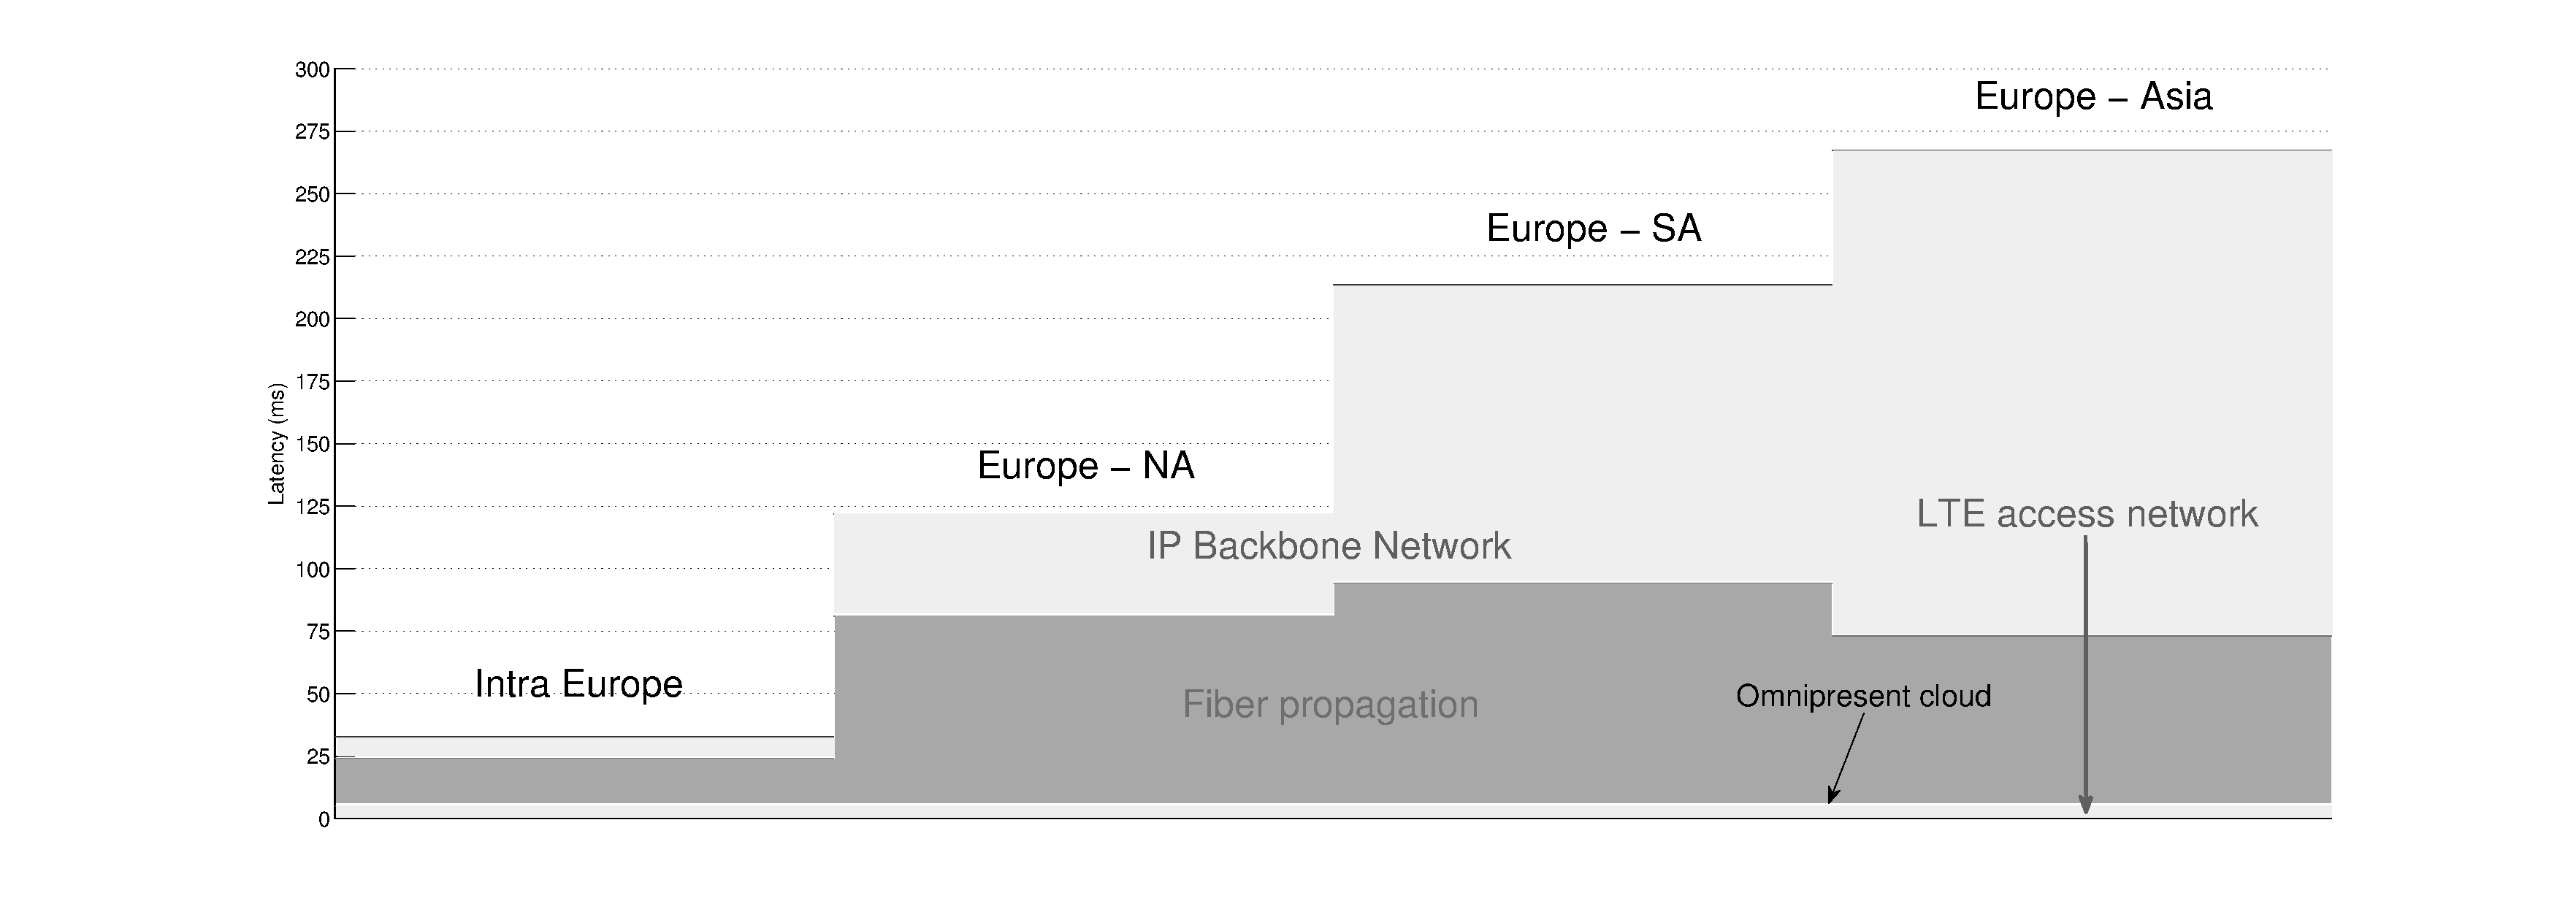
\includegraphics[height=0.12\paperheight]{omni_motivation.pdf} 
	\caption{IP Internet latency in western Europe \cite{BT_IP} over LTE \cite{blajic2006latency}}
	\label{fig:omni_motivation}
\end{figure}

Moving the cloud data centres closer to the IP backbone networks eliminates some of the additive latency on one side of the connection. Doing so, not only eliminate the propagation delay, but will over time, add more complexity to peripheries of the backbone as more severs nodes make their home there. 

The \xcloud remedies this latency challenge in a more sustainable way. By moving compute resources to the mobile networks, IP backbone network propagation and routing delays are eliminate without disrupting the Internet topology. The resulting distributed infrastructure is capable of delivering content and services at latencies less than 10 ms. 

The \xcloud will thus enable latency-sensitive services to be migrated to the cloud, such as, gaming, financial trading, process control, and most real-time human-machine interaction process.